\begin{figure*}[t]
    \centering
    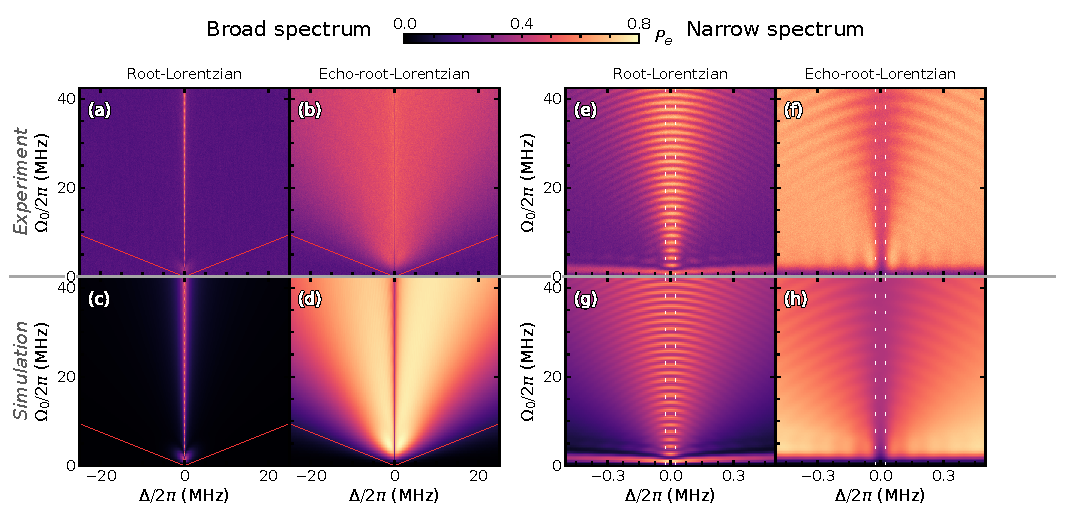
\includegraphics[width=0.88\textwidth]{../figures/paper/02_central_spectroscopy_experiment_simulation_variant.pdf}
    \caption{
Experimental and simulated spectroscopy for $L=20~\mu\mathrm{s}$ and
$c=0.005$. The left block (a)--(d) spans $50~\mathrm{MHz}$; the right block
(e)--(h) resolves the central $1~\mathrm{MHz}$. Within each block,
root-Lorentzian and echo-root-Lorentzian pulses occupy the left and right
columns, respectively, with experiment above three-level Lindblad simulations.
Red lines in (a)--(d) mark the linear high-drive half-width of the
constant-drive reference,
$\Delta/(2\pi)=\pm[\Omega_0/(2\pi)]\sqrt{T_1/T_2}$, using
$T_2=\EffectiveTTwo~\mu\mathrm{s}$. Thin white dashed lines in (e)--(h) mark
$\Delta/(2\pi)=\pm1/(2\pi T_2)$, enclosing the coherence-limited FWHM
$1/(\pi T_2)=\EffectiveCoherenceFwhm~\mathrm{kHz}$.
Both pulse shapes produce much narrower central spectral features than the
constant-drive reference. The root-Lorentzian response exhibits pronounced
coherent oscillations, whereas the echo response retains a narrow
resonance-centered depletion across the drive range. Residual high-drive
oscillations in the echo response are consistent with AC-Stark phase
accumulation, which is not reversed by the echo phase inversion.
    }
    \label{fig:robust-echo-spectroscopy}
\end{figure*}
